\documentclass[aspectratio=169,10pt]{beamer}

\usetheme{Madrid}
\usecolortheme{default}
\setbeamertemplate{navigation symbols}{}
\setbeamertemplate{footline}[frame number]

\usepackage{amsmath,amssymb,booktabs,mathtools}
\usepackage{graphicx}
\usepackage{hyperref}

\definecolor{positive}{HTML}{0173B2}
\definecolor{negative}{HTML}{DE8F05}
\definecolor{emphasis}{HTML}{029E73}
\definecolor{neutral}{gray}{0.55}
\newcommand{\pos}[1]{\textcolor{positive}{#1}}
\newcommand{\con}[1]{\textcolor{negative}{#1}}
\newcommand{\HL}[1]{\textcolor{emphasis}{#1}}

\title{Metallicity Histories in AuroraLF}
\subtitle{Representative halos ending at \texorpdfstring{$z=12.5$}{z=12.5}}
\author{Presenter: Zhu Hourui}
\institute{AuroraLF}
\date{May 19, 2026}

\begin{document}

\begin{frame}
  \titlepage
\end{frame}

\begin{frame}{Display Design}
\begin{columns}[T]
\column{0.46\textwidth}
\textbf{Question}
\begin{itemize}
\item Track enrichment along Monte Carlo MAHs.
\item Compare canonical, redshift-gated, and burst-gated top-heavy modes.
\item Keep UV/SFR physics fixed; use birth metallicity in the IMF gate.
\end{itemize}

\column{0.50\textwidth}
\textbf{Representative grid}
\begin{align*}
z_{\rm final} &= 12.5,\\
\log_{10} M_h(z_{\rm final}) &= 9,\ 10,\ 11,\ 12,\\
N_{\rm track} &= 1000,\qquad N_z=240 .
\end{align*}
\end{columns}
\vspace{2mm}
\begin{center}
\small Histories show median and $16$--$84$ percentile ranges across valid tracks.
\end{center}
\end{frame}

\begin{frame}{One-Zone Metal Reservoir}
\begin{columns}[T]
\column{0.50\textwidth}
\textbf{Reservoir and birth metallicity}
\begin{align*}
M_{{\rm gas},i} &= f_{\rm gas} f_b M_{h,i},\\
Z_{{\rm gas},i} &= \frac{M_{Z,i}}{M_{{\rm gas},i}},\\
Z_{{\rm birth},i} &=
\frac{M_{Z,i^-}}{M_{{\rm gas},i}Z_\odot}\,
10^{\mathcal{N}(0,\sigma_{\rm birth})}.
\end{align*}

\column{0.46\textwidth}
\textbf{Effective yield}
\begin{align*}
y_i &= y
\left[1+(m_{\rm TH}-1)I_{{\rm TH},i}\right]
10^{\mathcal{N}(0,\sigma_y)},\\
y &=0.02,\qquad m_{\rm TH}=1.28 .
\end{align*}
\end{columns}
\vspace{1mm}
\begin{align*}
\Delta M_{Z,i} =
y_i\Delta M_{\star,i}
+Z_{\rm in}\Delta M_{{\rm in},i}
-Z_{{\rm gas},i-1}\left[(1-R)+\eta_i\right]\Delta M_{\star,i}.
\end{align*}
\end{frame}

\begin{frame}{Top-Heavy Source-Time Gates}
\begin{columns}[T]
\column{0.50\textwidth}
\textbf{IMF flag}
\begin{align*}
I_{\rm TH} &=0
&& \text{canonical},\\
I_Z &=\mathbf{1}[Z_{\rm birth}\le0.05Z_\odot],\\
I_{\rm TH}^{z10} &=\mathbf{1}[z_{\rm src}\ge 10]I_Z,\\
t_{\rm grow} &= M_h/\dot M_h,\\
I_{\rm TH}^{\rm burst} &=I_{\rm TH}^{z10}\,
\mathbf{1}\!\left[t_{\rm grow}\le 50~{\rm Myr}\right].
\end{align*}

\column{0.45\textwidth}
\textbf{Displayed summaries}
\begin{align*}
{\rm median}\left[Z_{\rm gas}/Z_\odot\right]
&\quad \text{over active halos},\\
{\rm median}\left[Z_{\rm birth}/Z_\odot\right]
&\quad \text{over star-forming cells}.
\end{align*}
\begin{itemize}
\item Bands: 16--84 percentile range.
\item Same MAH seed per mass for all modes.
\end{itemize}
\end{columns}
\end{frame}

\begin{frame}{Yield Multiplier Calibration}
\begin{center}
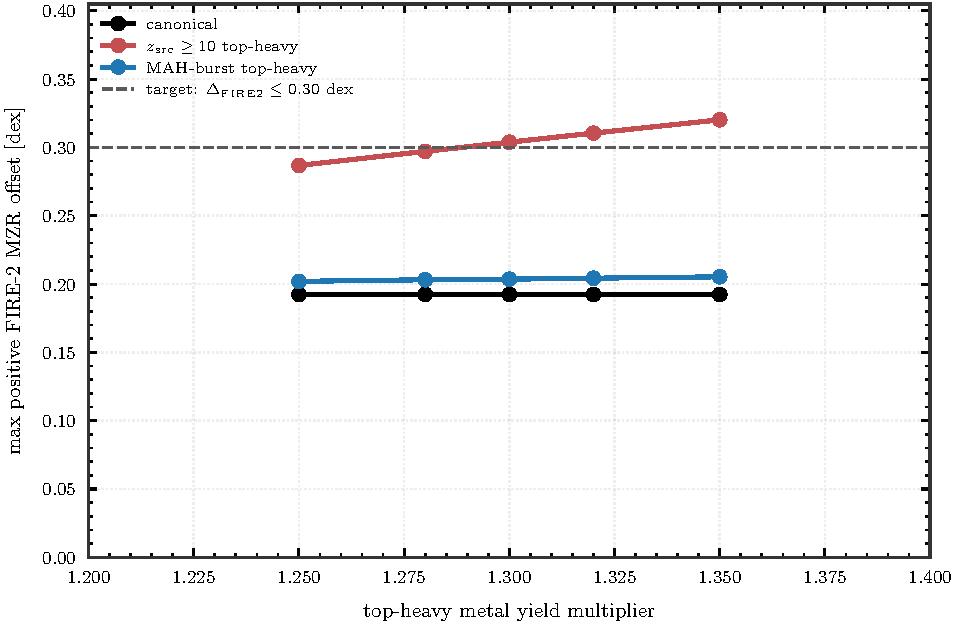
\includegraphics[height=0.78\textheight]{../assets/metal_yield_multiplier_sweep_z12p5.pdf}
\end{center}
\end{frame}

\begin{frame}{Metallicity Histories}
\begin{center}
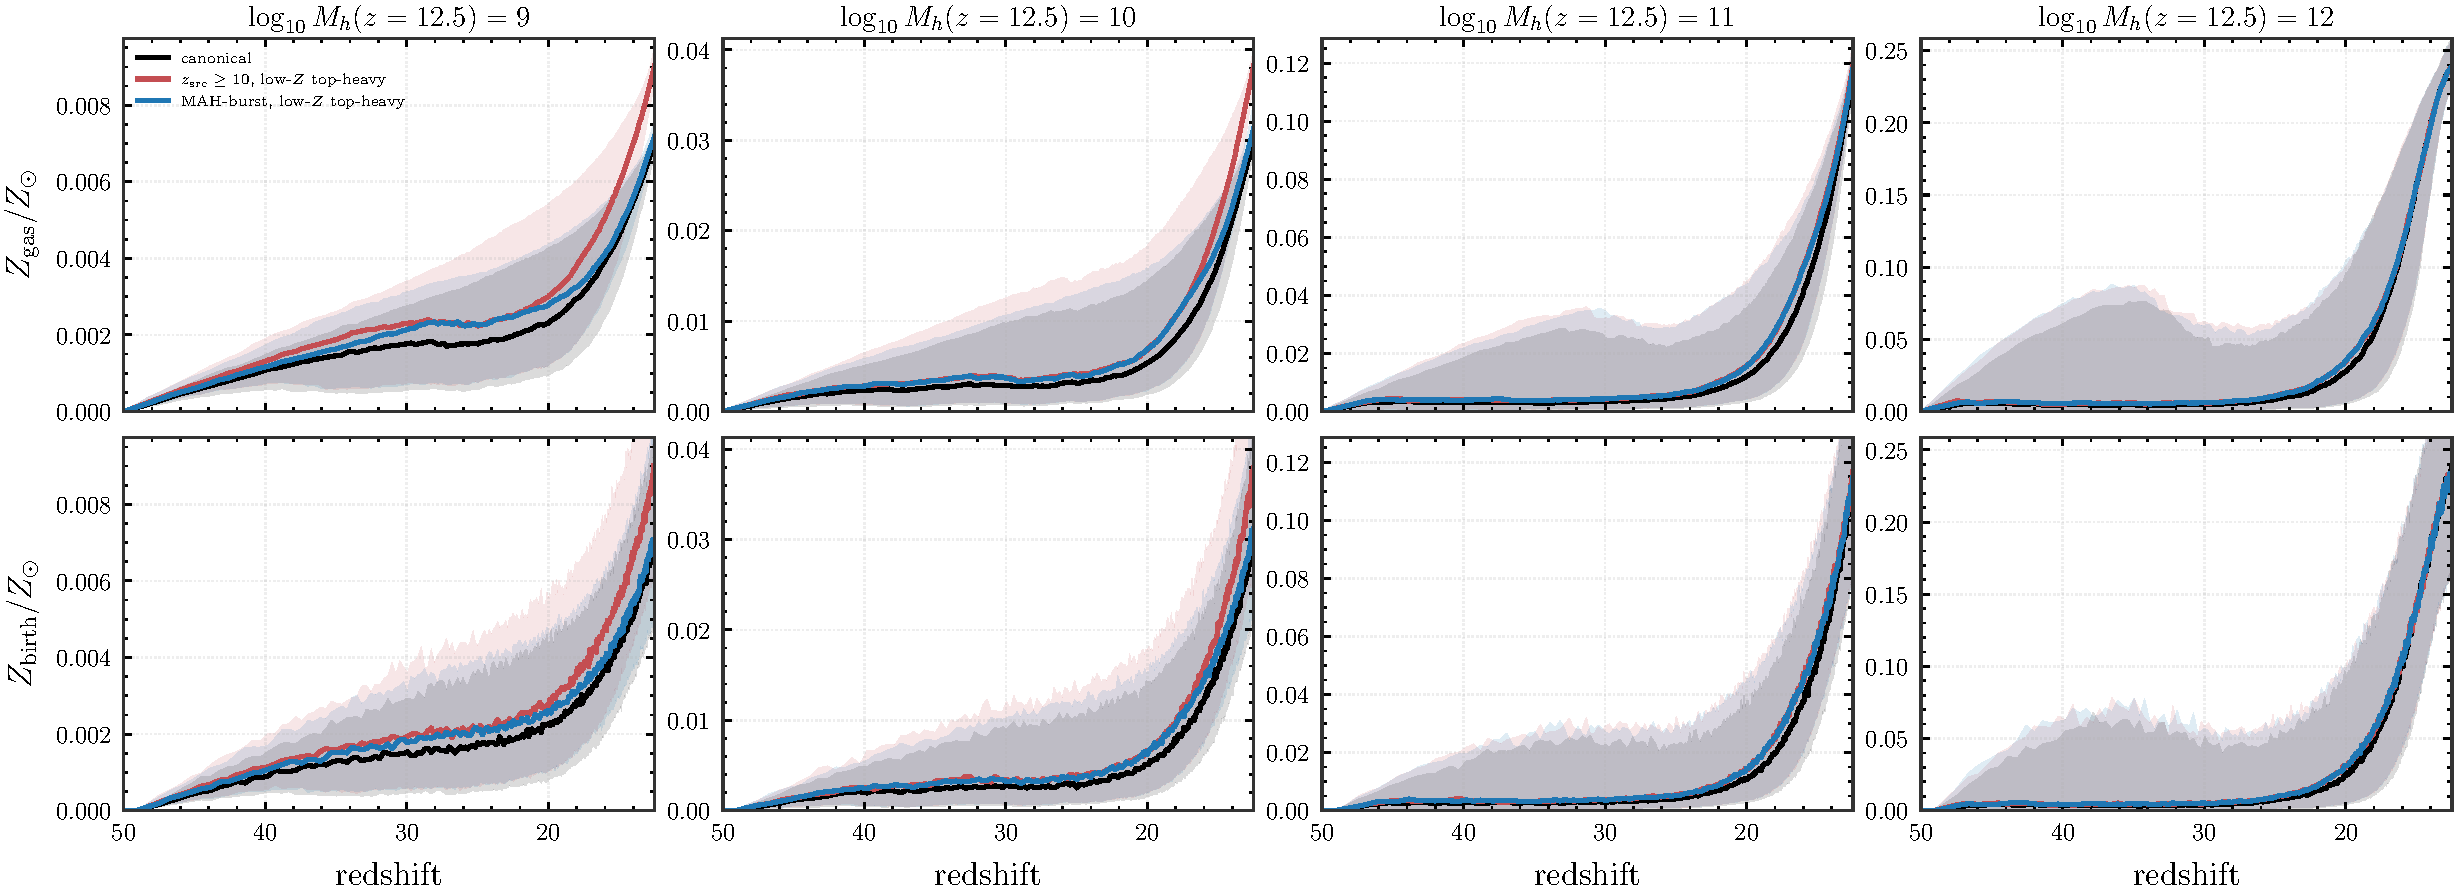
\includegraphics[width=\textwidth]{../assets/metallicity_history_z12p5.pdf}
\end{center}
\end{frame}

\begin{frame}{Literature MZR Check}
\begin{center}
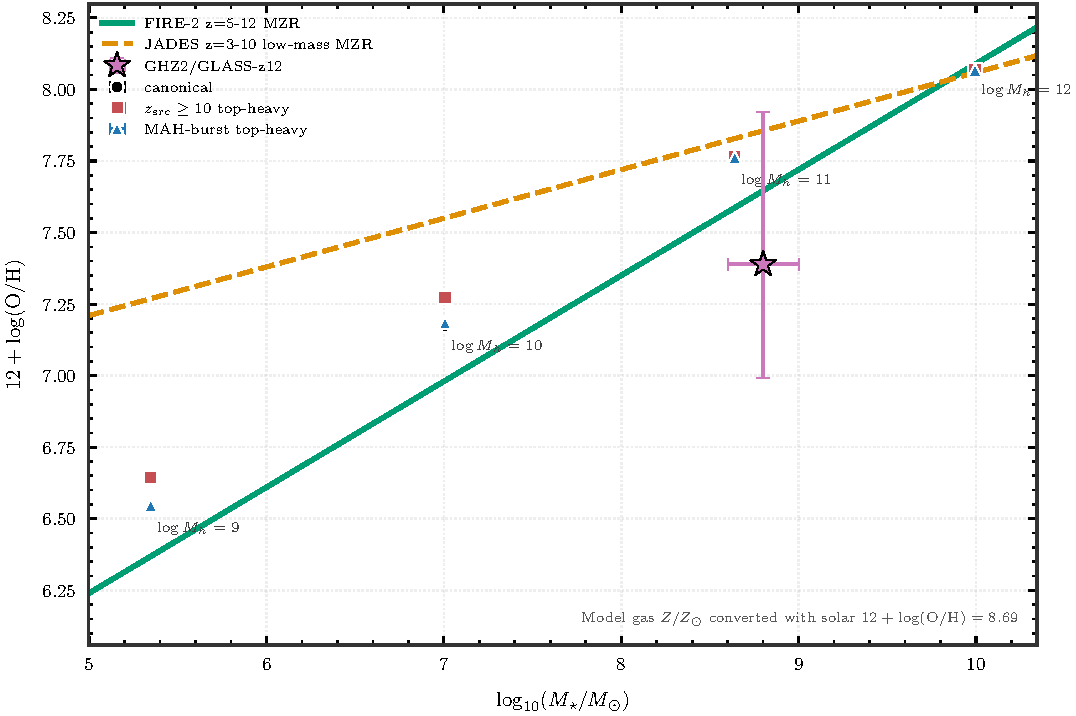
\includegraphics[height=0.78\textheight]{../assets/metallicity_mzr_literature_z12p5.pdf}
\end{center}
\end{frame}

\begin{frame}{Effect of the Low-Metallicity Gate}
\begin{center}
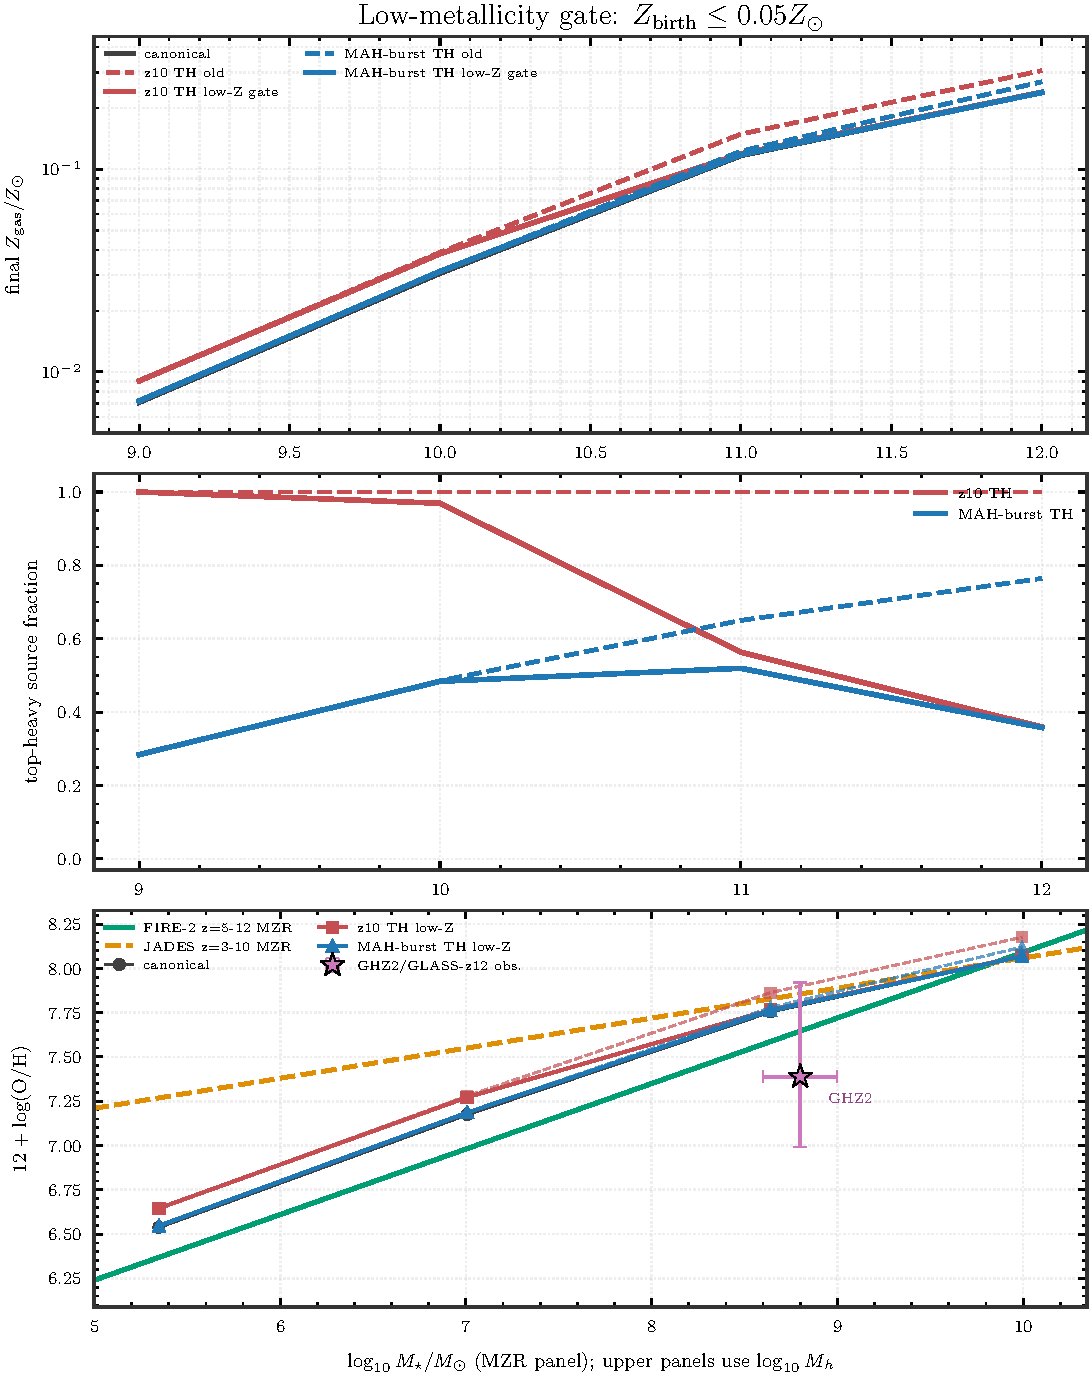
\includegraphics[height=0.80\textheight]{../assets/metallicity_lowzgate_comparison_z12p5.pdf}
\end{center}
\end{frame}

\begin{frame}{Final Gas Metallicity at \texorpdfstring{$z=12.5$}{z=12.5}}
\begin{center}
\small
\begin{tabular}{ccccc}
\toprule
$\log_{10}M_h$ &
canonical &
$z_{\rm src}\ge10$ TH &
MAH-burst TH &
$f_{\rm TH,src}$ (MAH)\\
\midrule
9  & 0.00705 & 0.00902 & 0.00719 & 0.284\\
10 & 0.0305  & 0.0389  & 0.0313  & 0.485\\
11 & 0.116   & 0.119   & 0.118   & 0.519\\
12 & 0.239   & 0.239   & 0.239   & 0.358\\
\bottomrule
\end{tabular}
\end{center}
\vspace{2mm}
\begin{columns}[T]
\column{0.47\textwidth}
\textbf{Mass trend}
\begin{itemize}
\item Final enrichment rises strongly with final halo mass.
\item High-mass MAHs enter the burst gate more often.
\end{itemize}
\column{0.47\textwidth}
\textbf{Mode trend}
\begin{itemize}
\item $z10$ is strongly suppressed once $Z_{\rm birth}>0.05Z_\odot$.
\item MAH-burst remains close to canonical at all four masses.
\end{itemize}
\end{columns}
\end{frame}

\begin{frame}{Interpretation}
\begin{itemize}
\item \HL{Low-Z gate}: top-heavy requires $Z_{\rm birth}\le0.05Z_\odot$.
\item \HL{High-mass halos}: $z10$ top-heavy source fraction falls from $1.00$ to $0.36$ at $\log M_h=12$.
\item \HL{MZR effect}: maximum positive FIRE-2 offset changes from $+0.297$ to $+0.290$ dex for $z10$.
\item \HL{JADES effect}: maximum positive JADES excess drops from $+0.117$ to $+0.010$ dex.
\item SFR and dust remain fixed; only SSP choice and metal yield use the new IMF gate.
\end{itemize}
\end{frame}

\begin{frame}{References}
\small
\begin{thebibliography}{9}
\bibitem{reed2007} Reed et al. 2007, halo mass function fitting functions.
\bibitem{curti2023} Curti et al. 2023, JADES low-mass MZR at $3<z<10$.
\bibitem{marszewski2024} Marszewski et al. 2024, FIRE-2 gas-phase MZR at $z=5$--12.
\bibitem{castellano2024} Castellano et al. 2024, GHZ2/GLASS-z12 metallicity at $z=12.33$.
\bibitem{bpass} Eldridge et al. 2017, BPASS stellar population synthesis.
\bibitem{bpass221} Stanway \& Eldridge 2018, BPASS v2.2 binary populations.
\bibitem{auroralf} AuroraLF local implementation,
\texttt{codex/topheavy-stochastic-metallicity}.
\end{thebibliography}
\end{frame}

\begin{frame}{Thank You}
\begin{center}
\Large
Metallicity histories are now available as per-track diagnostics for the
top-heavy IMF branches.
\end{center}
\end{frame}

\appendix

\begin{frame}{Backup: Output Files}
\small
\begin{tabular}{ll}
\toprule
Product & Prefix\\
\midrule
history outputs & \texttt{metallicity\_history\_z12p5\_mth1p28\_lowzgate\_20260519}\\
slide asset & \texttt{slides/assets/metallicity\_history\_z12p5.pdf}\\
MZR comparison & \texttt{metallicity\_mzr\_literature\_z12p5\_mth1p28\_lowzgate\_20260519}\\
old/new comparison & \texttt{metallicity\_lowzgate\_comparison\_z12p5\_mth1p28\_20260519}\\
\bottomrule
\end{tabular}
\end{frame}

\begin{frame}{Backup: Birth Metallicity at \texorpdfstring{$z=12.5$}{z=12.5}}
\begin{center}
\small
\begin{tabular}{cccc}
\toprule
$\log_{10}M_h$ &
canonical &
$z_{\rm src}\ge10$ TH &
MAH-burst TH\\
\midrule
9  & 0.00701 & 0.00889 & 0.00692\\
10 & 0.0298  & 0.0380  & 0.0312\\
11 & 0.117   & 0.117   & 0.115\\
12 & 0.238   & 0.233   & 0.234\\
\bottomrule
\end{tabular}
\end{center}
\vspace{2mm}
\small Birth metallicity is sampled only for star-forming source-time cells.
\end{frame}

\end{document}
